\part{Projektmanagement}

\chapter{Vorgehensmodell}


\chapter{Rollen und Verantwortlichkeiten}


\chapter{Risiken}\label{sec:risiken}


\chapter{Entwicklungsumgebung}


\section{Projektmanagement}
\section{Kommunikation}
Bei der Durchführung der Bachelorarbeit DAT wollten wir auf die Kommunikation per E-Mail verzichten. Wir haben unsere Informationen zwischen Mitarbeitern und Dozenten, wie zur Protokollierung der Sitzungen mittels \purl{http://slack.com} ausgetauscht. Slack bietet Team-Kommunikation auf hohem Niveau, mit der Möglichkeit Services wie GitHub oder Travis zu integrieren. So konnte an einem Zentralen Ort Bezug auf Commits und Build Results genommen werden. Durch die Verwendung eines dedizierten Tools zur Kommunikation konnte das E-Mail Postfach von Bachelor relevanten Themen frei gehalten werden und direkt Bezug auf konkrete Ereignisse genommen werden. \vref{fig:slack} \\

\begin{figure}[H]
	\centering
	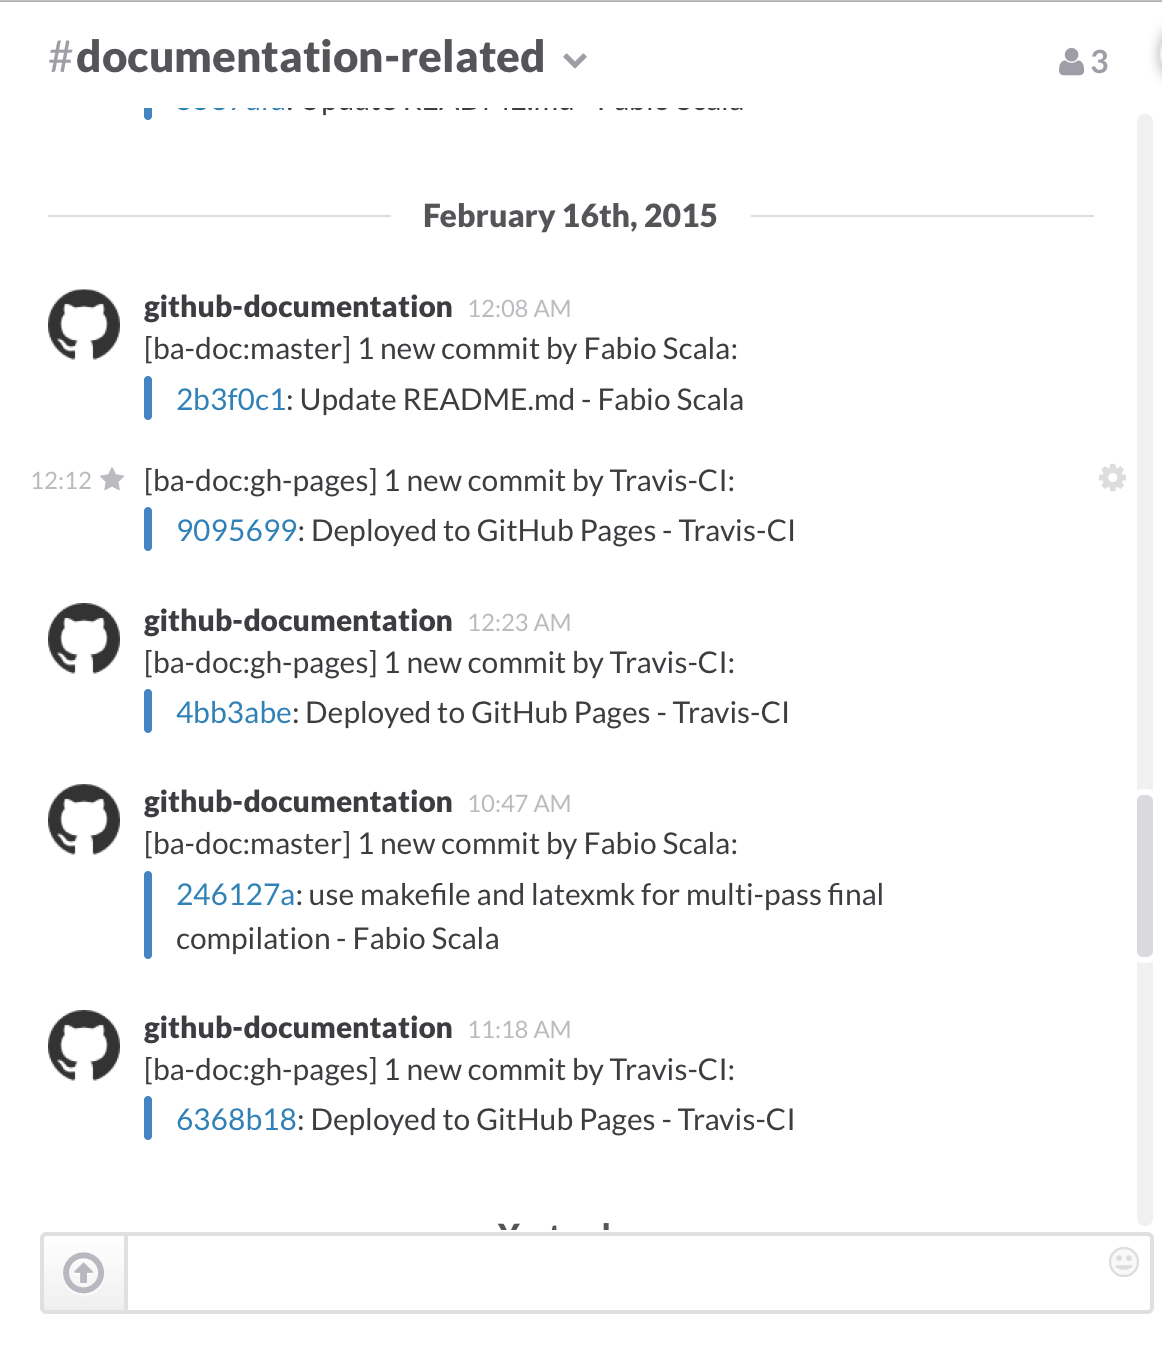
\includegraphics[width=0.5\linewidth]{fig/slack}
	\caption{Screenshot Slack}
	\label{fig:slack}
\end{figure}

\chapter{Qualitätsmanagement}

\section{Reviews}

Um die Qualität der umgesetzten Tasks zu erhöhen und sicherzustellen wurde ein Review-Prozess eingesetzt. Jeder Task darf erst abgeschlossen werden, wenn ein anderes Teammitglied das Resultat grob angeschaut und für gut befunden hat. Um diesen Prozess einzuhalten wurde ein eigener Jira-Workflow verwendet.

\begin{figure}
\centering
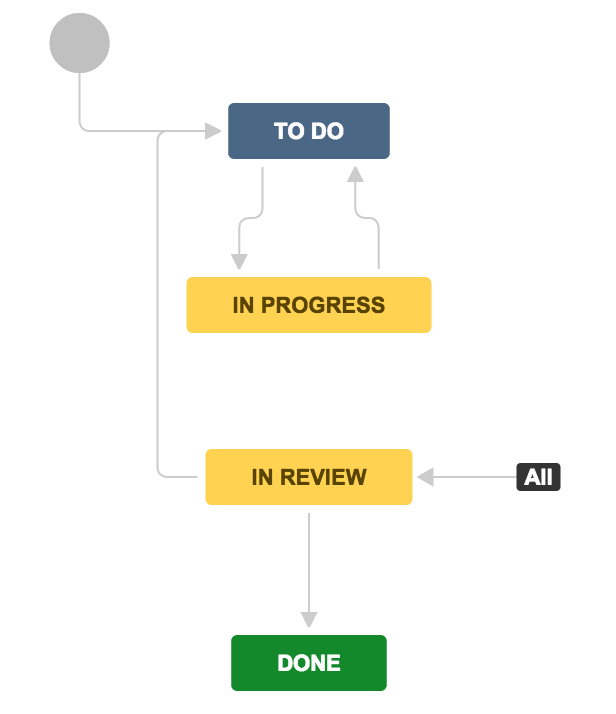
\includegraphics[width=0.7\linewidth]{content/projektmanagement/fig/jira-workflow}
\caption{Jira Review-Workflow}
\label{fig:jira-workflow}
\end{figure}

Der in \cref{fig:jira-workflow} dargestellte Prozess stellt sicher, dass alle Tasks erst in den Review Status versetzt werden müssen. Von diesem Status aus kann der Task entweder durch den Reviewer geschlossen oder zurück in den Status ''To Do'' versetzt werden, wobei bei letzterem der Tasks automatisch dem ursprünglichen Teammitglied zugewiesen wird.



\section{Tests}



\section{Coding-Richtlinien}


\subimport{sprints/}{sprints.tex}


